\section{Aufgabe 7}

\paragraph{a)} %\newline

Der Korrelationskoeffizient berechnet sich aus Formel \eqref{eqn:rho} und beträgt $\rho = \SI{0,8}{}$.
\begin{equation}
  \rho = \frac{\symup{Cov} (x, y)}{\sigma_x \cdot \sigma_y}
  \label{eqn:rho}
\end{equation}

\paragraph{b)} %\newline

Die 2D-Gaußverteilung sieht wie folgt aus:
\begin{equation*}
  f(x, y) = \frac{1}{2 \pi \sigma_x \sigma_y \sqrt{1-\rho}} \exp{\left(-\frac{1}{2(1-\rho^2)}\left(\frac{(x-\mu_x)^2}{\sigma^2_x} + \frac{(y-\mu_y)^2}{\sigma^2_y} - 2 \rho \frac{(x-\mu_x) (y-\mu_y)}{\sigma_x \sigma_y} \right)\right)} \overset{!}{=} \mathrm{const.}
\end{equation*}

Durch Umformung erhält man Gleichung \ref{eqn:ellips}. Diese ist ist eine Ellipsengleichung.
\begin{equation}
  \frac{(x-\mu_x)^2}{\sigma^2_x}+ \frac{(y-\mu_y)^2}{\sigma^2_y} - 2 \rho \frac{(x-\mu_x) (y-\mu_y)}{\sigma_x \sigma_y} = \mathrm{const.}
  \label{eqn:ellips}
\end{equation}

\paragraph{c)}

In Abbildung \ref{fig:ellips} ist die 2D-Gaußverteilung als Heatmap dargestellt.
Zusätzlich sind die Ellipse, bei der $f(x,y)$ auf das $\sfrac{1}{\sqrt{e}}$-fache seines Maximums abgefallen ist, und die Mittelwerte mit ihren Standardabweichungen eingezeichnet.
\begin{figure}[H]
  \centering
  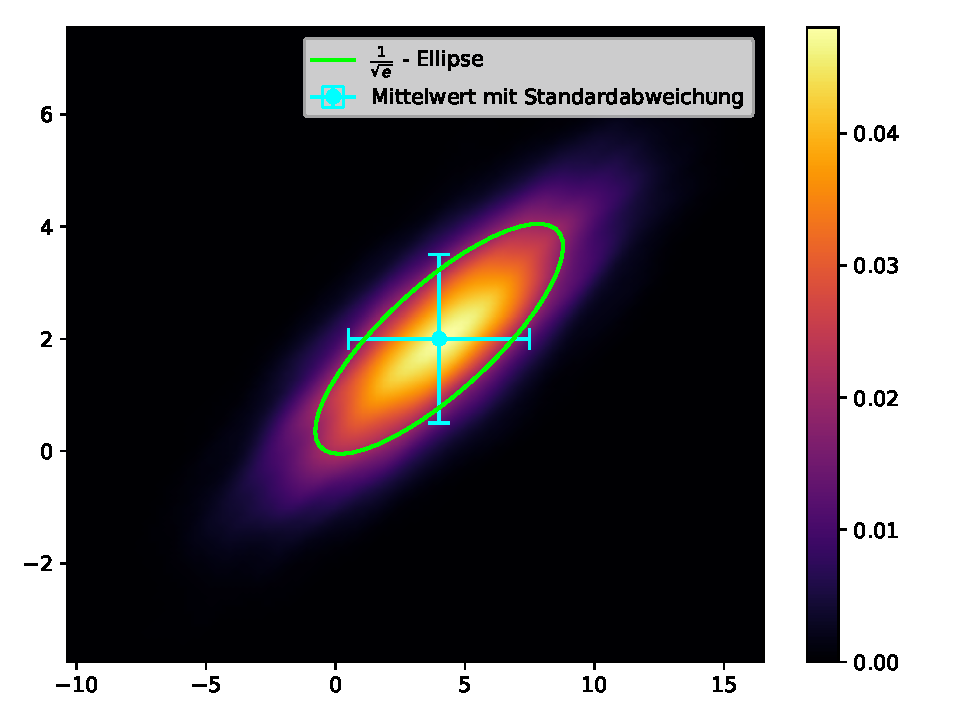
\includegraphics[width=\textwidth]{Aufgabe07/ellipse.pdf}
  \caption{2D-Gaußverteilung}
  \label{fig:ellips}
\end{figure}
